\documentclass[12pt,xcolor=dvipsnames]{beamer}
\usetheme{CambridgeUS}
\usecolortheme{whale}
\setbeamercolor{block title}{use=structure,fg=white,bg=blue!75!black}  
\setbeamercolor{block body}{use=structure,fg=black,bg=blue!5!white}
\setbeamercolor{frametitle}{bg=Blue}

\usepackage{hyperref}   
\usepackage{url}
\hypersetup{urlcolor=red}

\renewcommand{\bibname}{References}
\setbeamertemplate{bibliography item}{[\theenumiv]}

\usepackage{multicol}
\usepackage{verbatim} 
\usepackage{graphics}
\usepackage{graphicx}


%Basic Information
\title{Write your title here}
\author{Write your name Here}
\date{\today}

%--------------------------------------------------------------------------------------
%               TITLE PAGE (Slide 1)
%--------------------------------------------------------------------------------------
\begin{document}
\begin{frame}
\titlepage
\end{frame}
%--------------------------------------------------------------------------------------


%--------------------------------------------------------------------------------------
%               Outline
%--------------------------------------------------------------------------------------
\begin{frame}
\frametitle{Outline}
\begin{multicols}{2}
\tableofcontents[hideallsubsections]
\end{multicols}
\end{frame}

%--------------------------------------------------------------------------------------
%               Slide 1: Topic 1
%--------------------------------------------------------------------------------------
\section{Topic 1}
\begin{frame}[t]
\frametitle{Topic 1}
Write text here. \\
This is the first slide

For bulleted points use the following:\\
\begin{itemize}
 \item write point 1
 \item write poin 2
\end{itemize}

For numbered list use the following:\\
\begin{enumerate}
 \item write point 1
 \item write point 2
\end{enumerate}

\end{frame}

%--------------------------------------------------------------------------------------
%               Slide 2: Subtopic of Topic 1
%--------------------------------------------------------------------------------------

\subsection{sub topic of topic 1}
\begin{frame}[t]
\frametitle{Sub topic of topic 1}

\begin{center}
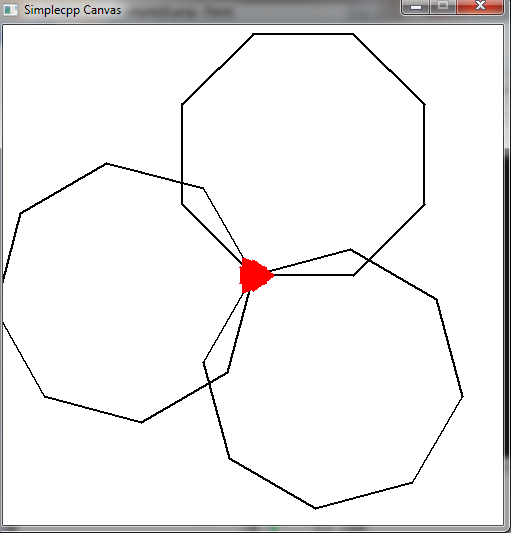
\includegraphics[height=3.5cm]{simple19.png}\\ % Insert your image it this way
Fig: SimpleCPP Output \cite{SimpleCPP-Windows}
\end{center}
\end{frame}

%--------------------------------------------------------------------------------------
%               Slide 3: Topic 2
%--------------------------------------------------------------------------------------
\section{Topic 2}
\begin{frame}[t]
\frametitle{Topic 2}
Use the following for creating a table \\
\begin{center}
\begin{tabular}{|c|c|c|}
 \hline
 No. & Name & Project \\
 \hline
 1 & Firuza & Code::Blocks \\
 \hline
 2 & Birundha & edX \\
 \hline
\end{tabular}
\end{center}
\end{frame}


%---------------------------------------------------------------------------------------
%     Final Slide - References
%--------------------------------------------------------------------------------------
\section{References}
\frametitle{References}
\begin{frame}[allowframebreaks]{References}
\bibliographystyle{ieeetr}
\bibliography{biblio}
\end{frame}
\end{document}
